% Created by tikzDevice version 0.12.6 on 2026-09-11 15:07:17
% !TEX encoding = UTF-8 Unicode
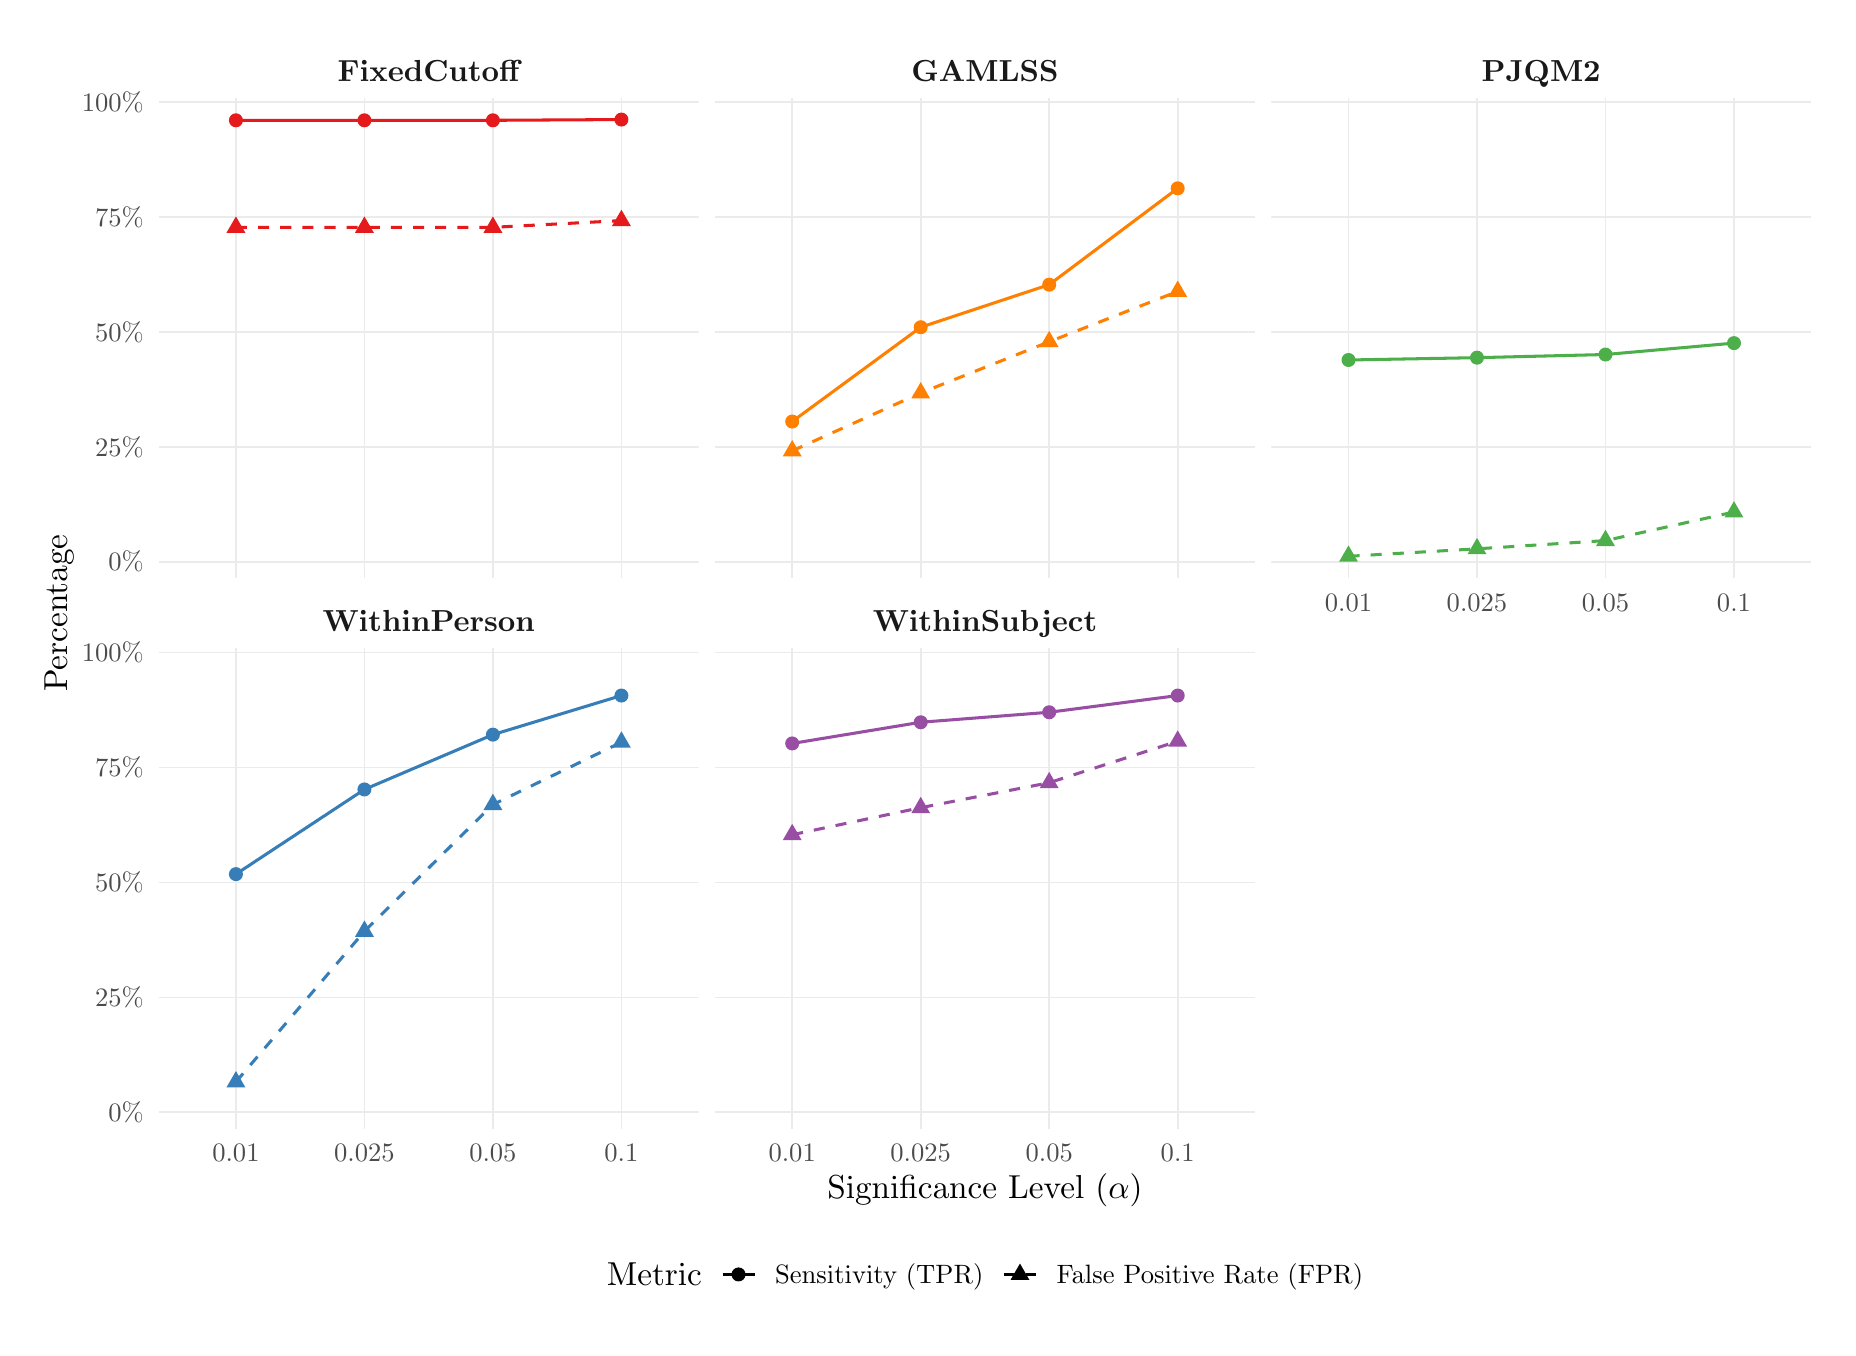
\begin{tikzpicture}[x=1pt,y=1pt]
\definecolor{fillColor}{RGB}{255,255,255}
\path[use as bounding box,fill=fillColor,fill opacity=0.00] (0,0) rectangle (650.43,469.75);
\begin{scope}
\path[clip] (  0.00,  0.00) rectangle (650.43,469.75);
\definecolor{fillColor}{RGB}{255,255,255}

\path[fill=fillColor] (  0.00,  0.00) rectangle (650.43,469.76);
\end{scope}
\begin{scope}
\path[clip] ( 47.39,270.84) rectangle (242.40,444.43);
\definecolor{drawColor}{gray}{0.92}

\path[draw=drawColor,line width= 0.6pt,line join=round] ( 47.39,276.75) --
	(242.40,276.75);

\path[draw=drawColor,line width= 0.6pt,line join=round] ( 47.39,318.27) --
	(242.40,318.27);

\path[draw=drawColor,line width= 0.6pt,line join=round] ( 47.39,359.79) --
	(242.40,359.79);

\path[draw=drawColor,line width= 0.6pt,line join=round] ( 47.39,401.31) --
	(242.40,401.31);

\path[draw=drawColor,line width= 0.6pt,line join=round] ( 47.39,442.83) --
	(242.40,442.83);

\path[draw=drawColor,line width= 0.6pt,line join=round] ( 75.25,270.84) --
	( 75.25,444.43);

\path[draw=drawColor,line width= 0.6pt,line join=round] (121.68,270.84) --
	(121.68,444.43);

\path[draw=drawColor,line width= 0.6pt,line join=round] (168.11,270.84) --
	(168.11,444.43);

\path[draw=drawColor,line width= 0.6pt,line join=round] (214.55,270.84) --
	(214.55,444.43);
\definecolor{drawColor}{RGB}{228,26,28}

\path[draw=drawColor,line width= 1.1pt,line join=round] ( 75.25,436.27) --
	(121.68,436.27) --
	(168.11,436.27) --
	(214.55,436.54);

\path[draw=drawColor,line width= 1.1pt,dash pattern=on 4pt off 4pt ,line join=round] ( 75.25,397.60) --
	(121.68,397.60) --
	(168.11,397.60) --
	(214.55,400.03);
\definecolor{fillColor}{RGB}{228,26,28}

\path[fill=fillColor] ( 75.25,436.27) circle (  2.53);

\path[fill=fillColor] ( 75.25,401.53) --
	( 78.66,395.63) --
	( 71.84,395.63) --
	cycle;

\path[fill=fillColor] (121.68,436.27) circle (  2.53);

\path[fill=fillColor] (121.68,401.53) --
	(125.09,395.63) --
	(118.28,395.63) --
	cycle;

\path[fill=fillColor] (168.11,436.27) circle (  2.53);

\path[fill=fillColor] (168.11,401.53) --
	(171.52,395.63) --
	(164.71,395.63) --
	cycle;

\path[fill=fillColor] (214.55,436.54) circle (  2.53);

\path[fill=fillColor] (214.55,403.96) --
	(217.95,398.06) --
	(211.14,398.06) --
	cycle;
\end{scope}
\begin{scope}
\path[clip] ( 47.39, 71.93) rectangle (242.40,245.51);
\definecolor{drawColor}{gray}{0.92}

\path[draw=drawColor,line width= 0.6pt,line join=round] ( 47.39, 77.83) --
	(242.40, 77.83);

\path[draw=drawColor,line width= 0.6pt,line join=round] ( 47.39,119.35) --
	(242.40,119.35);

\path[draw=drawColor,line width= 0.6pt,line join=round] ( 47.39,160.87) --
	(242.40,160.87);

\path[draw=drawColor,line width= 0.6pt,line join=round] ( 47.39,202.39) --
	(242.40,202.39);

\path[draw=drawColor,line width= 0.6pt,line join=round] ( 47.39,243.91) --
	(242.40,243.91);

\path[draw=drawColor,line width= 0.6pt,line join=round] ( 75.25, 71.93) --
	( 75.25,245.51);

\path[draw=drawColor,line width= 0.6pt,line join=round] (121.68, 71.93) --
	(121.68,245.51);

\path[draw=drawColor,line width= 0.6pt,line join=round] (168.11, 71.93) --
	(168.11,245.51);

\path[draw=drawColor,line width= 0.6pt,line join=round] (214.55, 71.93) --
	(214.55,245.51);
\definecolor{drawColor}{RGB}{55,126,184}

\path[draw=drawColor,line width= 1.1pt,line join=round] ( 75.25,163.88) --
	(121.68,194.48) --
	(168.11,214.28) --
	(214.55,228.41);

\path[draw=drawColor,line width= 1.1pt,dash pattern=on 4pt off 4pt ,line join=round] ( 75.25, 88.80) --
	(121.68,143.22) --
	(168.11,189.02) --
	(214.55,211.54);
\definecolor{fillColor}{RGB}{55,126,184}

\path[fill=fillColor] ( 75.25,163.88) circle (  2.53);

\path[fill=fillColor] ( 75.25, 92.73) --
	( 78.66, 86.83) --
	( 71.84, 86.83) --
	cycle;

\path[fill=fillColor] (121.68,194.48) circle (  2.53);

\path[fill=fillColor] (121.68,147.15) --
	(125.09,141.25) --
	(118.28,141.25) --
	cycle;

\path[fill=fillColor] (168.11,214.28) circle (  2.53);

\path[fill=fillColor] (168.11,192.96) --
	(171.52,187.05) --
	(164.71,187.05) --
	cycle;

\path[fill=fillColor] (214.55,228.41) circle (  2.53);

\path[fill=fillColor] (214.55,215.48) --
	(217.95,209.58) --
	(211.14,209.58) --
	cycle;
\end{scope}
\begin{scope}
\path[clip] (248.40,270.84) rectangle (443.42,444.43);
\definecolor{drawColor}{gray}{0.92}

\path[draw=drawColor,line width= 0.6pt,line join=round] (248.40,276.75) --
	(443.42,276.75);

\path[draw=drawColor,line width= 0.6pt,line join=round] (248.40,318.27) --
	(443.42,318.27);

\path[draw=drawColor,line width= 0.6pt,line join=round] (248.40,359.79) --
	(443.42,359.79);

\path[draw=drawColor,line width= 0.6pt,line join=round] (248.40,401.31) --
	(443.42,401.31);

\path[draw=drawColor,line width= 0.6pt,line join=round] (248.40,442.83) --
	(443.42,442.83);

\path[draw=drawColor,line width= 0.6pt,line join=round] (276.26,270.84) --
	(276.26,444.43);

\path[draw=drawColor,line width= 0.6pt,line join=round] (322.70,270.84) --
	(322.70,444.43);

\path[draw=drawColor,line width= 0.6pt,line join=round] (369.13,270.84) --
	(369.13,444.43);

\path[draw=drawColor,line width= 0.6pt,line join=round] (415.56,270.84) --
	(415.56,444.43);
\definecolor{drawColor}{RGB}{255,127,0}

\path[draw=drawColor,line width= 1.1pt,line join=round] (276.26,327.42) --
	(322.70,361.50) --
	(369.13,376.88) --
	(415.56,411.70);

\path[draw=drawColor,line width= 1.1pt,dash pattern=on 4pt off 4pt ,line join=round] (276.26,316.82) --
	(322.70,337.75) --
	(369.13,356.26) --
	(415.56,374.45);
\definecolor{fillColor}{RGB}{255,127,0}

\path[fill=fillColor] (276.26,327.42) circle (  2.53);

\path[fill=fillColor] (276.26,320.76) --
	(279.67,314.85) --
	(272.86,314.85) --
	cycle;

\path[fill=fillColor] (322.70,361.50) circle (  2.53);

\path[fill=fillColor] (322.70,341.68) --
	(326.10,335.78) --
	(319.29,335.78) --
	cycle;

\path[fill=fillColor] (369.13,376.88) circle (  2.53);

\path[fill=fillColor] (369.13,360.20) --
	(372.53,354.29) --
	(365.72,354.29) --
	cycle;

\path[fill=fillColor] (415.56,411.70) circle (  2.53);

\path[fill=fillColor] (415.56,378.39) --
	(418.97,372.48) --
	(412.15,372.48) --
	cycle;
\end{scope}
\begin{scope}
\path[clip] (248.40, 71.93) rectangle (443.42,245.51);
\definecolor{drawColor}{gray}{0.92}

\path[draw=drawColor,line width= 0.6pt,line join=round] (248.40, 77.83) --
	(443.42, 77.83);

\path[draw=drawColor,line width= 0.6pt,line join=round] (248.40,119.35) --
	(443.42,119.35);

\path[draw=drawColor,line width= 0.6pt,line join=round] (248.40,160.87) --
	(443.42,160.87);

\path[draw=drawColor,line width= 0.6pt,line join=round] (248.40,202.39) --
	(443.42,202.39);

\path[draw=drawColor,line width= 0.6pt,line join=round] (248.40,243.91) --
	(443.42,243.91);

\path[draw=drawColor,line width= 0.6pt,line join=round] (276.26, 71.93) --
	(276.26,245.51);

\path[draw=drawColor,line width= 0.6pt,line join=round] (322.70, 71.93) --
	(322.70,245.51);

\path[draw=drawColor,line width= 0.6pt,line join=round] (369.13, 71.93) --
	(369.13,245.51);

\path[draw=drawColor,line width= 0.6pt,line join=round] (415.56, 71.93) --
	(415.56,245.51);
\definecolor{drawColor}{RGB}{152,78,163}

\path[draw=drawColor,line width= 1.1pt,line join=round] (276.26,211.10) --
	(322.70,218.76) --
	(369.13,222.37) --
	(415.56,228.41);

\path[draw=drawColor,line width= 1.1pt,dash pattern=on 4pt off 4pt ,line join=round] (276.26,178.12) --
	(322.70,187.89) --
	(369.13,196.91) --
	(415.56,211.91);
\definecolor{fillColor}{RGB}{152,78,163}

\path[fill=fillColor] (276.26,211.10) circle (  2.53);

\path[fill=fillColor] (276.26,182.06) --
	(279.67,176.16) --
	(272.86,176.16) --
	cycle;

\path[fill=fillColor] (322.70,218.76) circle (  2.53);

\path[fill=fillColor] (322.70,191.82) --
	(326.10,185.92) --
	(319.29,185.92) --
	cycle;

\path[fill=fillColor] (369.13,222.37) circle (  2.53);

\path[fill=fillColor] (369.13,200.84) --
	(372.53,194.94) --
	(365.72,194.94) --
	cycle;

\path[fill=fillColor] (415.56,228.41) circle (  2.53);

\path[fill=fillColor] (415.56,215.84) --
	(418.97,209.94) --
	(412.15,209.94) --
	cycle;
\end{scope}
\begin{scope}
\path[clip] (449.42,270.84) rectangle (644.43,444.43);
\definecolor{drawColor}{gray}{0.92}

\path[draw=drawColor,line width= 0.6pt,line join=round] (449.42,276.75) --
	(644.43,276.75);

\path[draw=drawColor,line width= 0.6pt,line join=round] (449.42,318.27) --
	(644.43,318.27);

\path[draw=drawColor,line width= 0.6pt,line join=round] (449.42,359.79) --
	(644.43,359.79);

\path[draw=drawColor,line width= 0.6pt,line join=round] (449.42,401.31) --
	(644.43,401.31);

\path[draw=drawColor,line width= 0.6pt,line join=round] (449.42,442.83) --
	(644.43,442.83);

\path[draw=drawColor,line width= 0.6pt,line join=round] (477.28,270.84) --
	(477.28,444.43);

\path[draw=drawColor,line width= 0.6pt,line join=round] (523.71,270.84) --
	(523.71,444.43);

\path[draw=drawColor,line width= 0.6pt,line join=round] (570.14,270.84) --
	(570.14,444.43);

\path[draw=drawColor,line width= 0.6pt,line join=round] (616.57,270.84) --
	(616.57,444.43);
\definecolor{drawColor}{RGB}{77,175,74}

\path[draw=drawColor,line width= 1.1pt,line join=round] (477.28,349.66) --
	(523.71,350.50) --
	(570.14,351.64) --
	(616.57,355.76);

\path[draw=drawColor,line width= 1.1pt,dash pattern=on 4pt off 4pt ,line join=round] (477.28,278.73) --
	(523.71,281.43) --
	(570.14,284.40) --
	(616.57,294.73);
\definecolor{fillColor}{RGB}{77,175,74}

\path[fill=fillColor] (477.28,349.66) circle (  2.53);

\path[fill=fillColor] (477.28,282.67) --
	(480.68,276.77) --
	(473.87,276.77) --
	cycle;

\path[fill=fillColor] (523.71,350.50) circle (  2.53);

\path[fill=fillColor] (523.71,285.37) --
	(527.12,279.47) --
	(520.30,279.47) --
	cycle;

\path[fill=fillColor] (570.14,351.64) circle (  2.53);

\path[fill=fillColor] (570.14,288.33) --
	(573.55,282.43) --
	(566.73,282.43) --
	cycle;

\path[fill=fillColor] (616.57,355.76) circle (  2.53);

\path[fill=fillColor] (616.57,298.66) --
	(619.98,292.76) --
	(613.16,292.76) --
	cycle;
\end{scope}
\begin{scope}
\path[clip] ( 47.39,245.51) rectangle (242.40,264.84);
\definecolor{drawColor}{gray}{0.10}

\node[text=drawColor,anchor=base,inner sep=0pt, outer sep=0pt, scale=  1.10] at (144.90,251.38) {\bfseries WithinPerson};
\end{scope}
\begin{scope}
\path[clip] (248.40,245.51) rectangle (443.42,264.84);
\definecolor{drawColor}{gray}{0.10}

\node[text=drawColor,anchor=base,inner sep=0pt, outer sep=0pt, scale=  1.10] at (345.91,251.38) {\bfseries WithinSubject};
\end{scope}
\begin{scope}
\path[clip] ( 47.39,444.43) rectangle (242.40,463.75);
\definecolor{drawColor}{gray}{0.10}

\node[text=drawColor,anchor=base,inner sep=0pt, outer sep=0pt, scale=  1.10] at (144.90,450.29) {\bfseries FixedCutoff};
\end{scope}
\begin{scope}
\path[clip] (248.40,444.43) rectangle (443.42,463.75);
\definecolor{drawColor}{gray}{0.10}

\node[text=drawColor,anchor=base,inner sep=0pt, outer sep=0pt, scale=  1.10] at (345.91,450.29) {\bfseries GAMLSS};
\end{scope}
\begin{scope}
\path[clip] (449.42,444.43) rectangle (644.43,463.75);
\definecolor{drawColor}{gray}{0.10}

\node[text=drawColor,anchor=base,inner sep=0pt, outer sep=0pt, scale=  1.10] at (546.92,450.29) {\bfseries PJQM2};
\end{scope}
\begin{scope}
\path[clip] (  0.00,  0.00) rectangle (650.43,469.75);
\definecolor{drawColor}{gray}{0.30}

\node[text=drawColor,anchor=base,inner sep=0pt, outer sep=0pt, scale=  0.96] at ( 75.25, 59.92) {0.01};

\node[text=drawColor,anchor=base,inner sep=0pt, outer sep=0pt, scale=  0.96] at (121.68, 59.92) {0.025};

\node[text=drawColor,anchor=base,inner sep=0pt, outer sep=0pt, scale=  0.96] at (168.11, 59.92) {0.05};

\node[text=drawColor,anchor=base,inner sep=0pt, outer sep=0pt, scale=  0.96] at (214.55, 59.92) {0.1};
\end{scope}
\begin{scope}
\path[clip] (  0.00,  0.00) rectangle (650.43,469.75);
\definecolor{drawColor}{gray}{0.30}

\node[text=drawColor,anchor=base,inner sep=0pt, outer sep=0pt, scale=  0.96] at (276.26, 59.92) {0.01};

\node[text=drawColor,anchor=base,inner sep=0pt, outer sep=0pt, scale=  0.96] at (322.70, 59.92) {0.025};

\node[text=drawColor,anchor=base,inner sep=0pt, outer sep=0pt, scale=  0.96] at (369.13, 59.92) {0.05};

\node[text=drawColor,anchor=base,inner sep=0pt, outer sep=0pt, scale=  0.96] at (415.56, 59.92) {0.1};
\end{scope}
\begin{scope}
\path[clip] (  0.00,  0.00) rectangle (650.43,469.75);
\definecolor{drawColor}{gray}{0.30}

\node[text=drawColor,anchor=base,inner sep=0pt, outer sep=0pt, scale=  0.96] at (477.28,258.83) {0.01};

\node[text=drawColor,anchor=base,inner sep=0pt, outer sep=0pt, scale=  0.96] at (523.71,258.83) {0.025};

\node[text=drawColor,anchor=base,inner sep=0pt, outer sep=0pt, scale=  0.96] at (570.14,258.83) {0.05};

\node[text=drawColor,anchor=base,inner sep=0pt, outer sep=0pt, scale=  0.96] at (616.57,258.83) {0.1};
\end{scope}
\begin{scope}
\path[clip] (  0.00,  0.00) rectangle (650.43,469.75);
\definecolor{drawColor}{gray}{0.30}

\node[text=drawColor,anchor=base east,inner sep=0pt, outer sep=0pt, scale=  0.96] at ( 41.99,273.44) {0\%};

\node[text=drawColor,anchor=base east,inner sep=0pt, outer sep=0pt, scale=  0.96] at ( 41.99,314.96) {25\%};

\node[text=drawColor,anchor=base east,inner sep=0pt, outer sep=0pt, scale=  0.96] at ( 41.99,356.48) {50\%};

\node[text=drawColor,anchor=base east,inner sep=0pt, outer sep=0pt, scale=  0.96] at ( 41.99,398.00) {75\%};

\node[text=drawColor,anchor=base east,inner sep=0pt, outer sep=0pt, scale=  0.96] at ( 41.99,439.52) {100\%};
\end{scope}
\begin{scope}
\path[clip] (  0.00,  0.00) rectangle (650.43,469.75);
\definecolor{drawColor}{gray}{0.30}

\node[text=drawColor,anchor=base east,inner sep=0pt, outer sep=0pt, scale=  0.96] at ( 41.99, 74.53) {0\%};

\node[text=drawColor,anchor=base east,inner sep=0pt, outer sep=0pt, scale=  0.96] at ( 41.99,116.05) {25\%};

\node[text=drawColor,anchor=base east,inner sep=0pt, outer sep=0pt, scale=  0.96] at ( 41.99,157.57) {50\%};

\node[text=drawColor,anchor=base east,inner sep=0pt, outer sep=0pt, scale=  0.96] at ( 41.99,199.09) {75\%};

\node[text=drawColor,anchor=base east,inner sep=0pt, outer sep=0pt, scale=  0.96] at ( 41.99,240.61) {100\%};
\end{scope}
\begin{scope}
\path[clip] (  0.00,  0.00) rectangle (650.43,469.75);
\definecolor{drawColor}{RGB}{0,0,0}

\node[text=drawColor,anchor=base,inner sep=0pt, outer sep=0pt, scale=  1.20] at (345.91, 46.79) {Significance Level ($\alpha$)};
\end{scope}
\begin{scope}
\path[clip] (  0.00,  0.00) rectangle (650.43,469.75);
\definecolor{drawColor}{RGB}{0,0,0}

\node[text=drawColor,rotate= 90.00,anchor=base,inner sep=0pt, outer sep=0pt, scale=  1.20] at ( 14.26,258.18) {Percentage};
\end{scope}
\begin{scope}
\path[clip] (  0.00,  0.00) rectangle (650.43,469.75);
\definecolor{drawColor}{RGB}{0,0,0}

\node[text=drawColor,anchor=base west,inner sep=0pt, outer sep=0pt, scale=  1.20] at (209.29, 15.09) {Metric};
\end{scope}
\begin{scope}
\path[clip] (  0.00,  0.00) rectangle (650.43,469.75);
\definecolor{drawColor}{RGB}{0,0,0}

\path[draw=drawColor,line width= 1.1pt,line join=round] (251.09, 19.23) -- (262.65, 19.23);
\definecolor{fillColor}{RGB}{0,0,0}

\path[fill=fillColor] (256.87, 19.23) circle (  2.53);
\end{scope}
\begin{scope}
\path[clip] (  0.00,  0.00) rectangle (650.43,469.75);
\definecolor{drawColor}{RGB}{0,0,0}

\path[draw=drawColor,line width= 1.1pt,dash pattern=on 4pt off 4pt ,line join=round] (352.78, 19.23) -- (364.34, 19.23);
\definecolor{fillColor}{RGB}{0,0,0}

\path[fill=fillColor] (358.56, 23.16) --
	(361.97, 17.26) --
	(355.15, 17.26) --
	cycle;
\end{scope}
\begin{scope}
\path[clip] (  0.00,  0.00) rectangle (650.43,469.75);
\definecolor{drawColor}{RGB}{0,0,0}

\node[text=drawColor,anchor=base west,inner sep=0pt, outer sep=0pt, scale=  0.96] at (270.10, 15.92) {Sensitivity (TPR)};
\end{scope}
\begin{scope}
\path[clip] (  0.00,  0.00) rectangle (650.43,469.75);
\definecolor{drawColor}{RGB}{0,0,0}

\node[text=drawColor,anchor=base west,inner sep=0pt, outer sep=0pt, scale=  0.96] at (371.79, 15.92) {False Positive Rate (FPR)};
\end{scope}
\end{tikzpicture}
